% !TeX root = Architekturdokument.tex

\clearpage

\section{Modularisierung}
Für die Modularisierung wird zuerst ein mögliches Grobentwurf entworfen. Zuletzt wird aus dem Grobentwurf der Feinentwurf. Bei der Modularisierung spielen zwei Faktoren eine sehr große Rolle. Zum einen sollten die Module so entworfen werden, dass Geheimnisse in dem Modul eingeschlossen sind und sich nicht auf die Schnittstellen des Moduls auswirken. Zum anderen sollte darauf geachtet werden, wie sich welche Anforderung an das System verändern kann. Basierend auf diesen beiden Faktoren kann eine gute Modularisierung entstehen. Das Ziel ist es Module zu identifizieren, die möglichst stabile Schnittstellen haben und Geheimnisse enthalten und verstecken. Also gilt es änderungsanfällige Stellen genauso, wie Geheimnisse weg zu kapseln. Dadurch soll letztendlich sicher gestellt werden, dass Änderungen in möglichst wenig Modulen angewendet werden müssen. 

\vspace{6pt}

Die Modularisierung bzw. die Architektur lässt sich nicht in wenig Diagrammen festhalten. Wir haben uns dazu entschieden für die verschiedenen Sichten die folgenden Diagrammtypen zu benutzen. \textbf{UML-Paketdiagramm} und das \textbf{UML-Komponentendiagramm}.

\newpage

\subsection{Grobentwurf}
Wir haben die Folgenden Module ausgearbeitet.

\vspace{12pt}

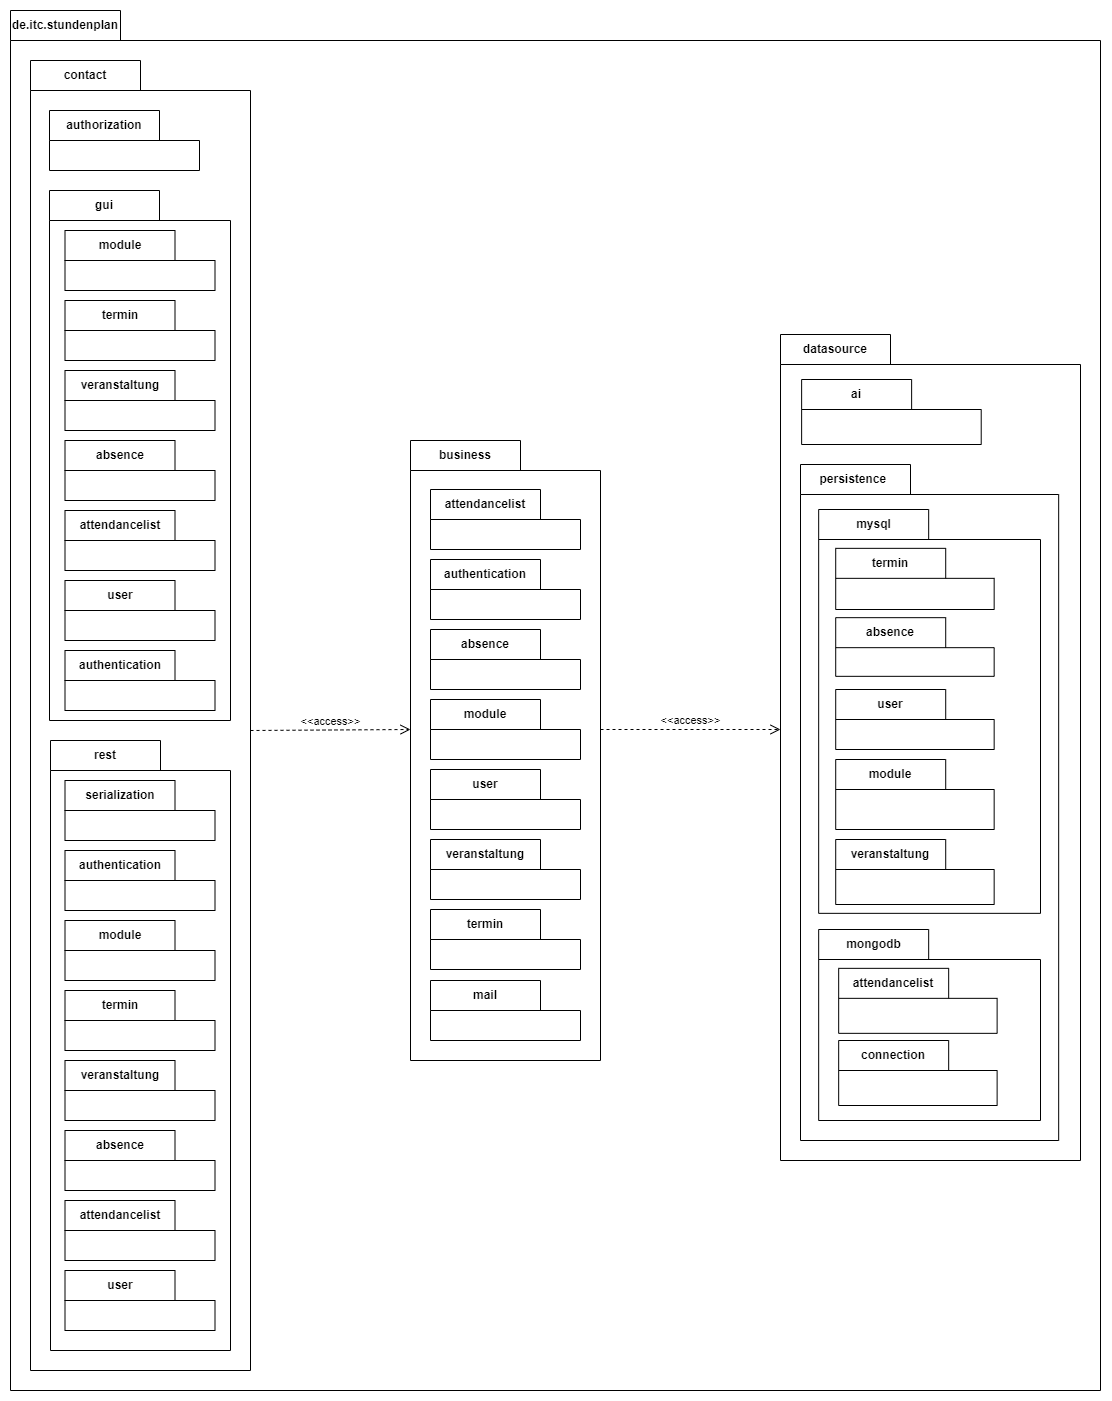
\includegraphics[width=\textwidth]{Paketdiagramm}

\newpage

\includegraphics[width=\textwidth]{KomponentendiagrammV2}

\newpage

\subsection{Feinentwurf}

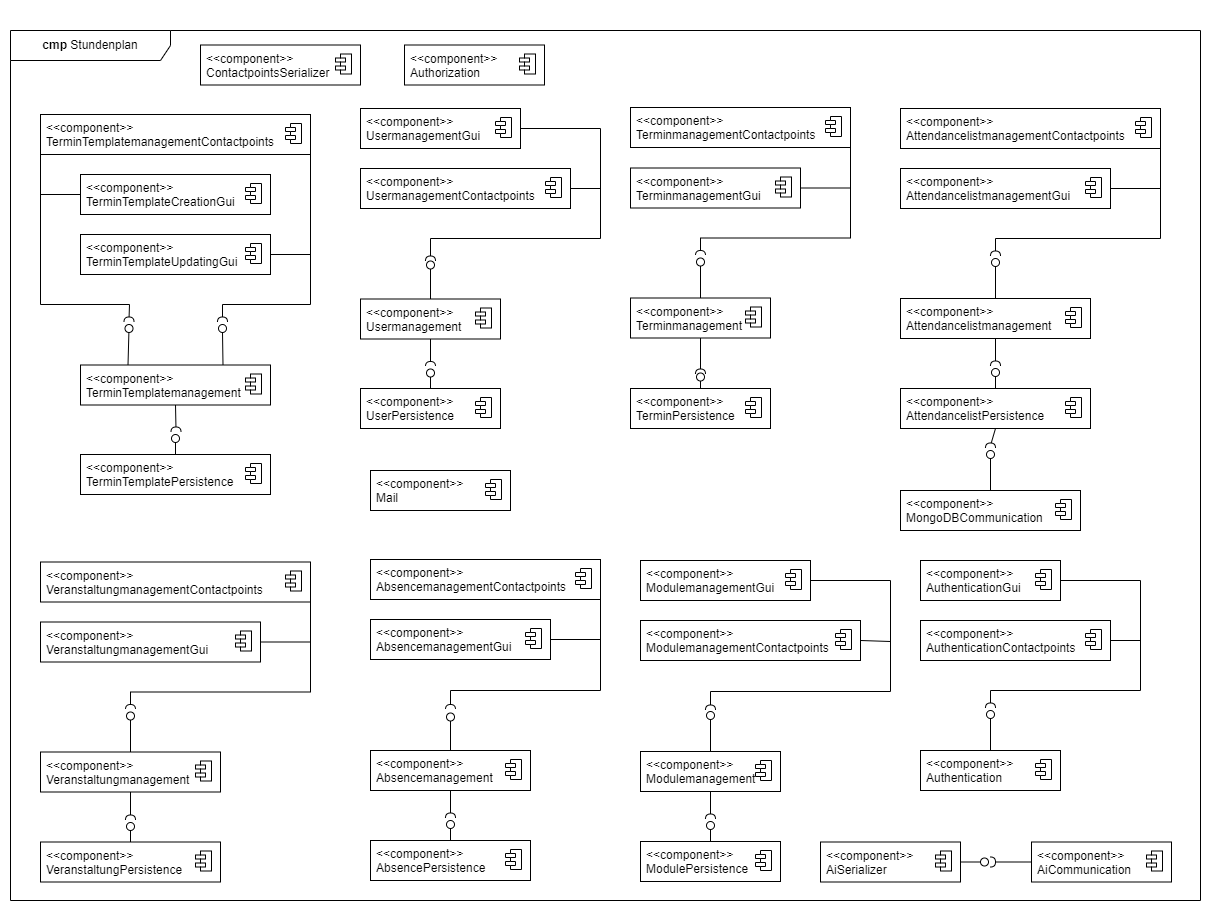
\includegraphics[width=\textwidth]{KomponentendiagrammV1_2}